% Vilnius University beamer template
% Created in 2024 by Joana Katina
% Adapted for final bachelor thesis defense

\documentclass[12pt]{beamer}

\renewcommand{\figurename}{}
\renewcommand{\tablename}{}
\renewcommand\thefigure{\arabic{figure} pav.}
\renewcommand\thetable{\arabic{table} lentelė.}

\usepackage{graphicx}
\usepackage{booktabs}
\usepackage{array}
\usepackage{caption}
\usepackage{hyperref}
\usepackage{iftex}
\usepackage{tikz}
\usetikzlibrary{positioning, arrows.meta}

\usetheme{Madrid}
\setbeamerfont{title}{size=\large}
\setbeamerfont{author}{size=\small}
\setbeamerfont{date}{size=\small}

\title[]{TurtleBot Burger robotui skirtų aplinkos išžvalgymo algoritmų palyginimas realiose sąlygose}
\subtitle[]{Bakalauro baigiamasis darbas}
\author[Gvidas Bačianskas]{Gvidas Bačianskas}
\date{Vilnius -- 2026}

\addtobeamertemplate{author}{}{Darbo vadovas: prof. dr. Virginijus Marcinkevičius\par}
\addtobeamertemplate{author}{}{Darbo recenzentas: doc. dr. Valentas Gružauskas\par}

\setbeamertemplate{navigation symbols}{}
\titlegraphic{}

\usepackage{VUMIF}
\ifLuaTeX
    \usepackage{fontspec}
    \setsansfont{Latin Modern Sans}
    \setmainfont{Latin Modern Roman}
\else
    \usepackage[T1]{fontenc}
    \usepackage[utf8]{inputenc}
\fi

\newcommand{\smallgap}{\vspace{0.18cm}}
\newcommand{\metricbest}[1]{\textbf{#1}}

\begin{document}

% 1. Titulinis
\begin{frame}
    \titlepage
\end{frame}

% 2. Problema ir tikslas
\begin{frame}{Problema ir tikslas}
    \textbf{Tyrimo problema:}
    
    \vspace{0.1cm}
    \begin{itemize}
        \item Skirtingais išžvalgymo sprendimų principais pagrįsti algoritmai gali nevienodai veikti skirtingos geometrijos vidaus patalpose ir realaus TurtleBot Burger roboto apribojimų sąlygomis.
    \end{itemize}

    \smallgap
    \textbf{Darbo tikslas:}
    \begin{itemize}
        \item Palyginti pasirinktus aplinkos išžvalgymo algoritmus, įgyvendintus vienoje ROS 2 ir TurtleBot Burger roboto architektūroje, taikant palyginamas realių vidaus patalpų eksperimentų sąlygas.
    \end{itemize}
\end{frame}

% 3. Tyrimo metodika
\begin{frame}{Tyrimo metodika}
    \begin{columns}[onlytextwidth]
        \column{0.52\textwidth}
        \textbf{Lyginamas sprendimas:}
        \begin{itemize}
            \item aukšto lygio išžvalgymo tikslo parinkimas;
            \item ne žemo lygio kelio planavimas.
        \end{itemize}

        \smallgap
        \textbf{Bendra infrastruktūra:}
        \begin{itemize}
            \item tas pats pagrindinis ciklas;
            \item ta pati Nav2 tikslų siuntimo sąsaja;
            \item tas pats metrikų registravimas.
        \end{itemize}
        \column{0.45\textwidth}
        \begin{figure}
            \centering
            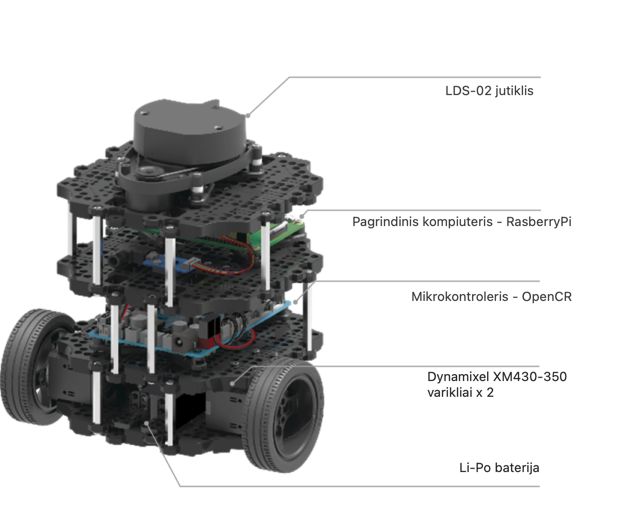
\includegraphics[width=0.85\textwidth]{images/final/TurtleBot.png}
            \caption{TurtleBot3 Burger}
        \end{figure}
    \end{columns}
\end{frame}

% 4. Architektūra
\begin{frame}{Sistemos architektūra}
    \begin{columns}[onlytextwidth]
        \column{0.43\textwidth}
        \textbf{Pagrindinės dalys:}
        \begin{itemize}
            \item TurtleBot Burger robotas;
            \item ROS 2 mazgai;
            \item SLAM Toolbox;
            \item Nav2 navigacija;
            \item išžvalgymo strategijos.
        \end{itemize}

        \smallgap
        Algoritmas parenka tikslą, o judėjimą iki jo vykdo Nav2.
        \column{0.57\textwidth}
        \begin{figure}
            \centering
            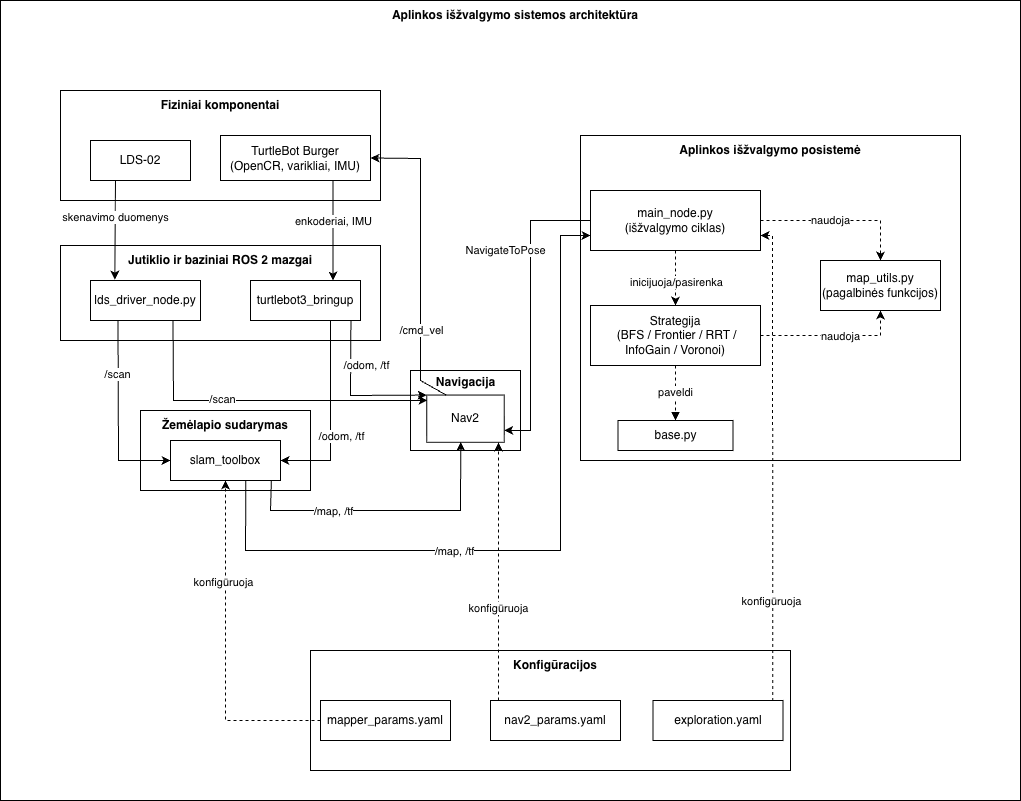
\includegraphics[width=0.98\textwidth]{images/final/sysarch.png}
            \caption{Programinės sistemos architektūra}
        \end{figure}
    \end{columns}
\end{frame}

% 5. Algoritmai
\begin{frame}{Lyginti algoritmai}
    \begin{table}
        \centering
        \scriptsize
        \begin{tabular}{p{0.32\textwidth}p{0.58\textwidth}}
            \toprule
            \textbf{Algoritmas} & \textbf{Tikslo parinkimo principas} \\
            \midrule
            BFS & Paieška per žinomą laisvą erdvę iki pirmos tinkamos viršūnės. \\
            Artimiausia riba & Pasirenkama mažiausiu atstumu pasiekiama riba. \\
            RRT & Atsitiktinai plečiamas medis, kandidatai vertinami pagal informaciją ir kainą. \\
            Informacijos prieaugis & Vertinamas tikėtinas naujos informacijos kiekis ir judėjimo kaina. \\
            Voronoi & Naudojama laisvos erdvės geometrinė struktūra ir kelias per Voronoi keteras. \\
            \bottomrule
        \end{tabular}
    \end{table}
\end{frame}

% 6. Eksperimentinės aplinkos
\begin{frame}{Eksperimentinės aplinkos}
    \begin{columns}[onlytextwidth]
        \column{0.33\textwidth}
        \begin{figure}
            \centering
            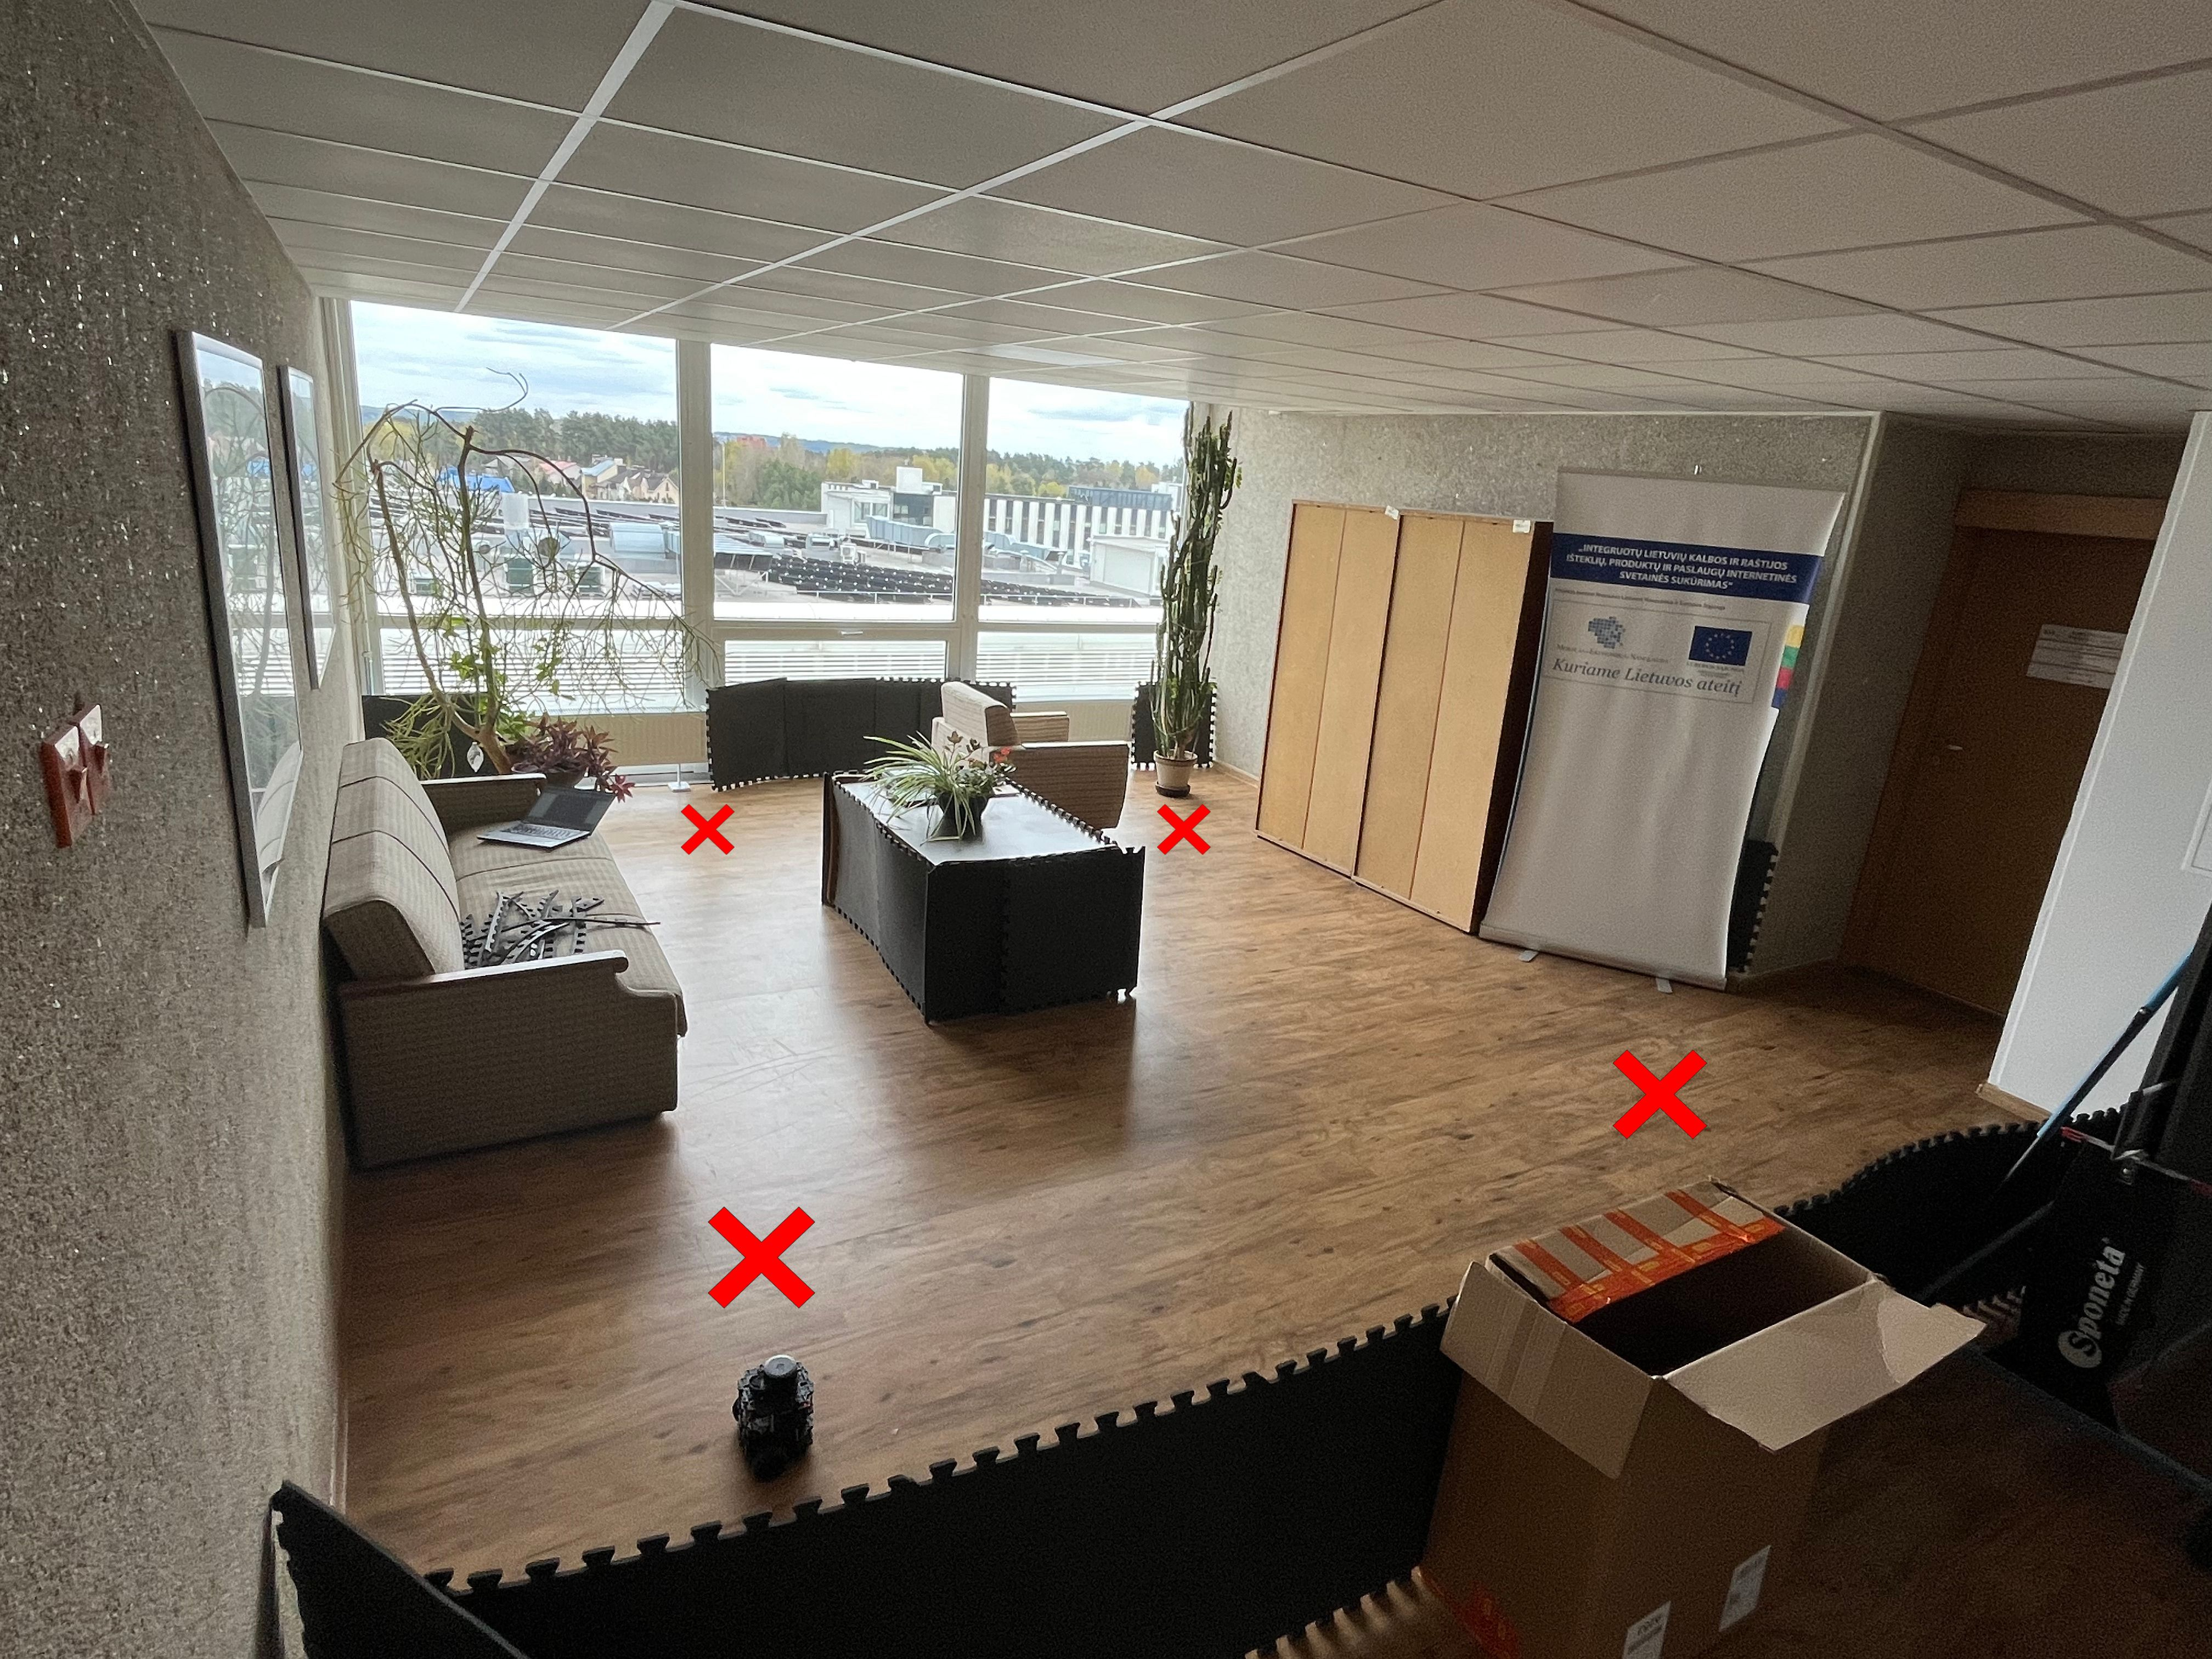
\includegraphics[height=0.37\textheight,width=\textwidth,keepaspectratio]{images/final/kamb1_marks.jpg}
            \caption{\scriptsize Kambarys su objektais}
        \end{figure}
        \column{0.33\textwidth}
        \begin{figure}
            \centering
            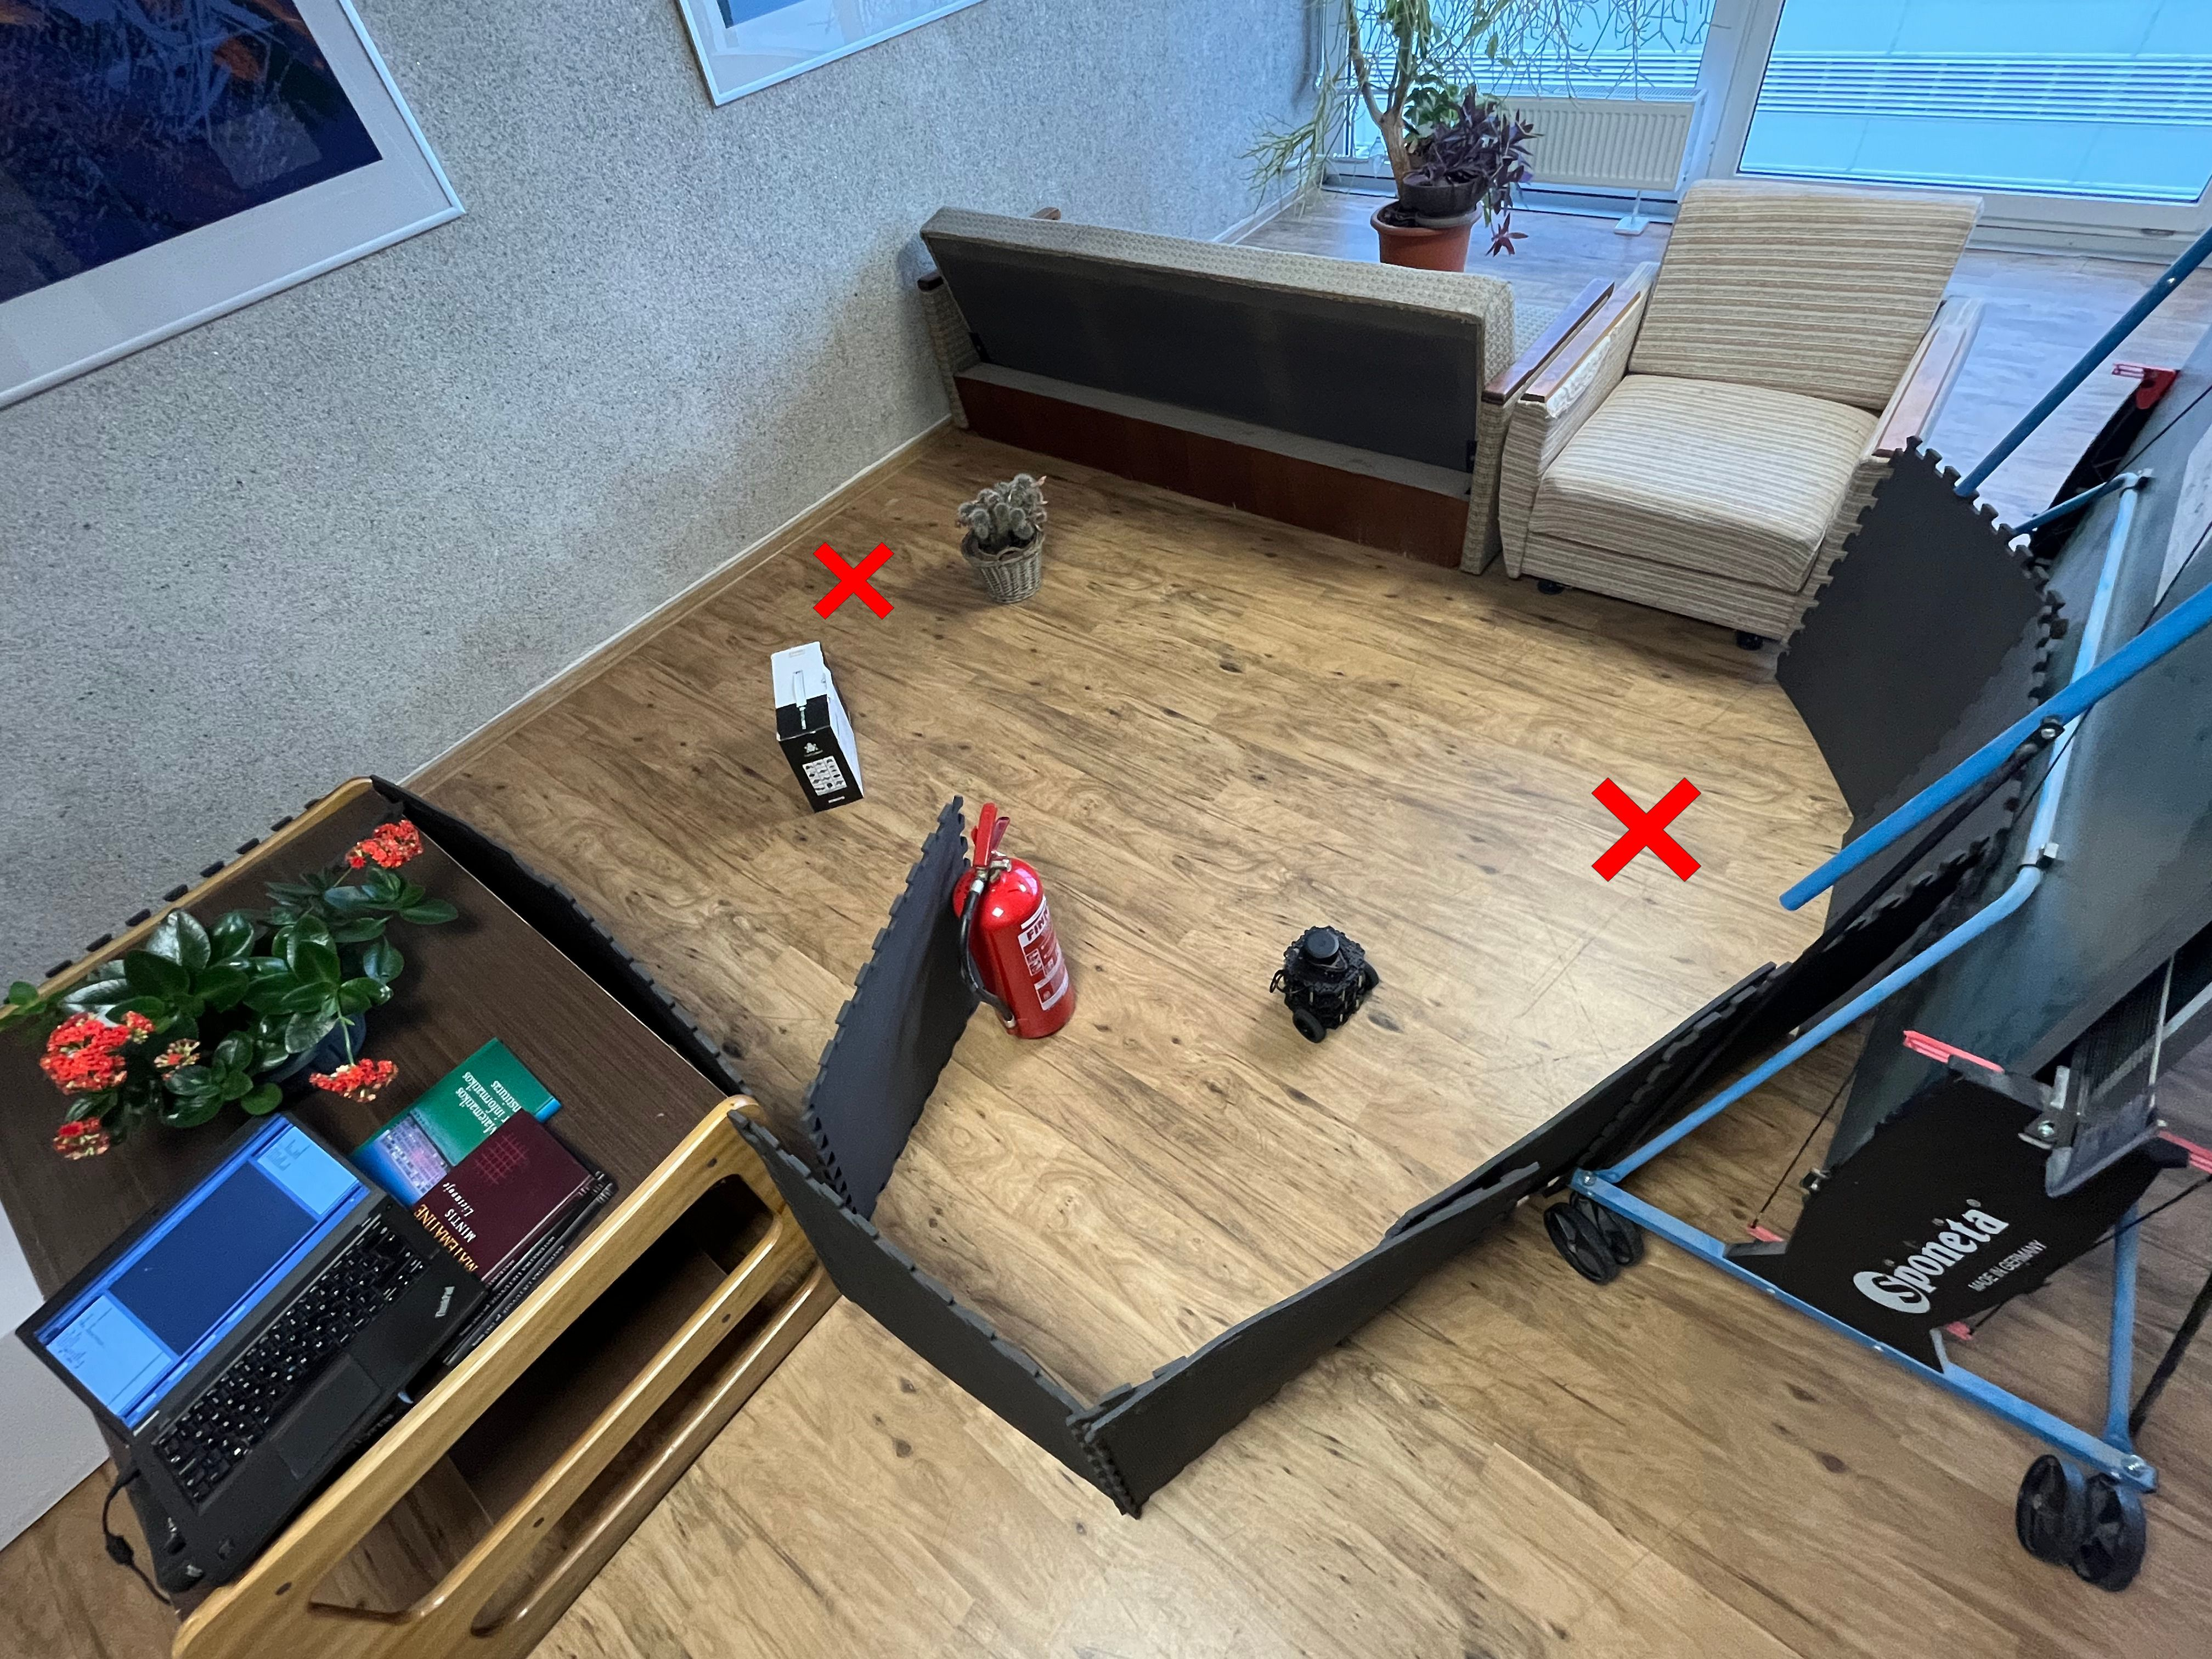
\includegraphics[height=0.37\textheight,width=\textwidth,keepaspectratio]{images/final/kamb2_marks.jpg}
            \caption{\scriptsize Patalpos su siauru praėjimu}
        \end{figure}
        \column{0.33\textwidth}
        \begin{figure}
            \centering
            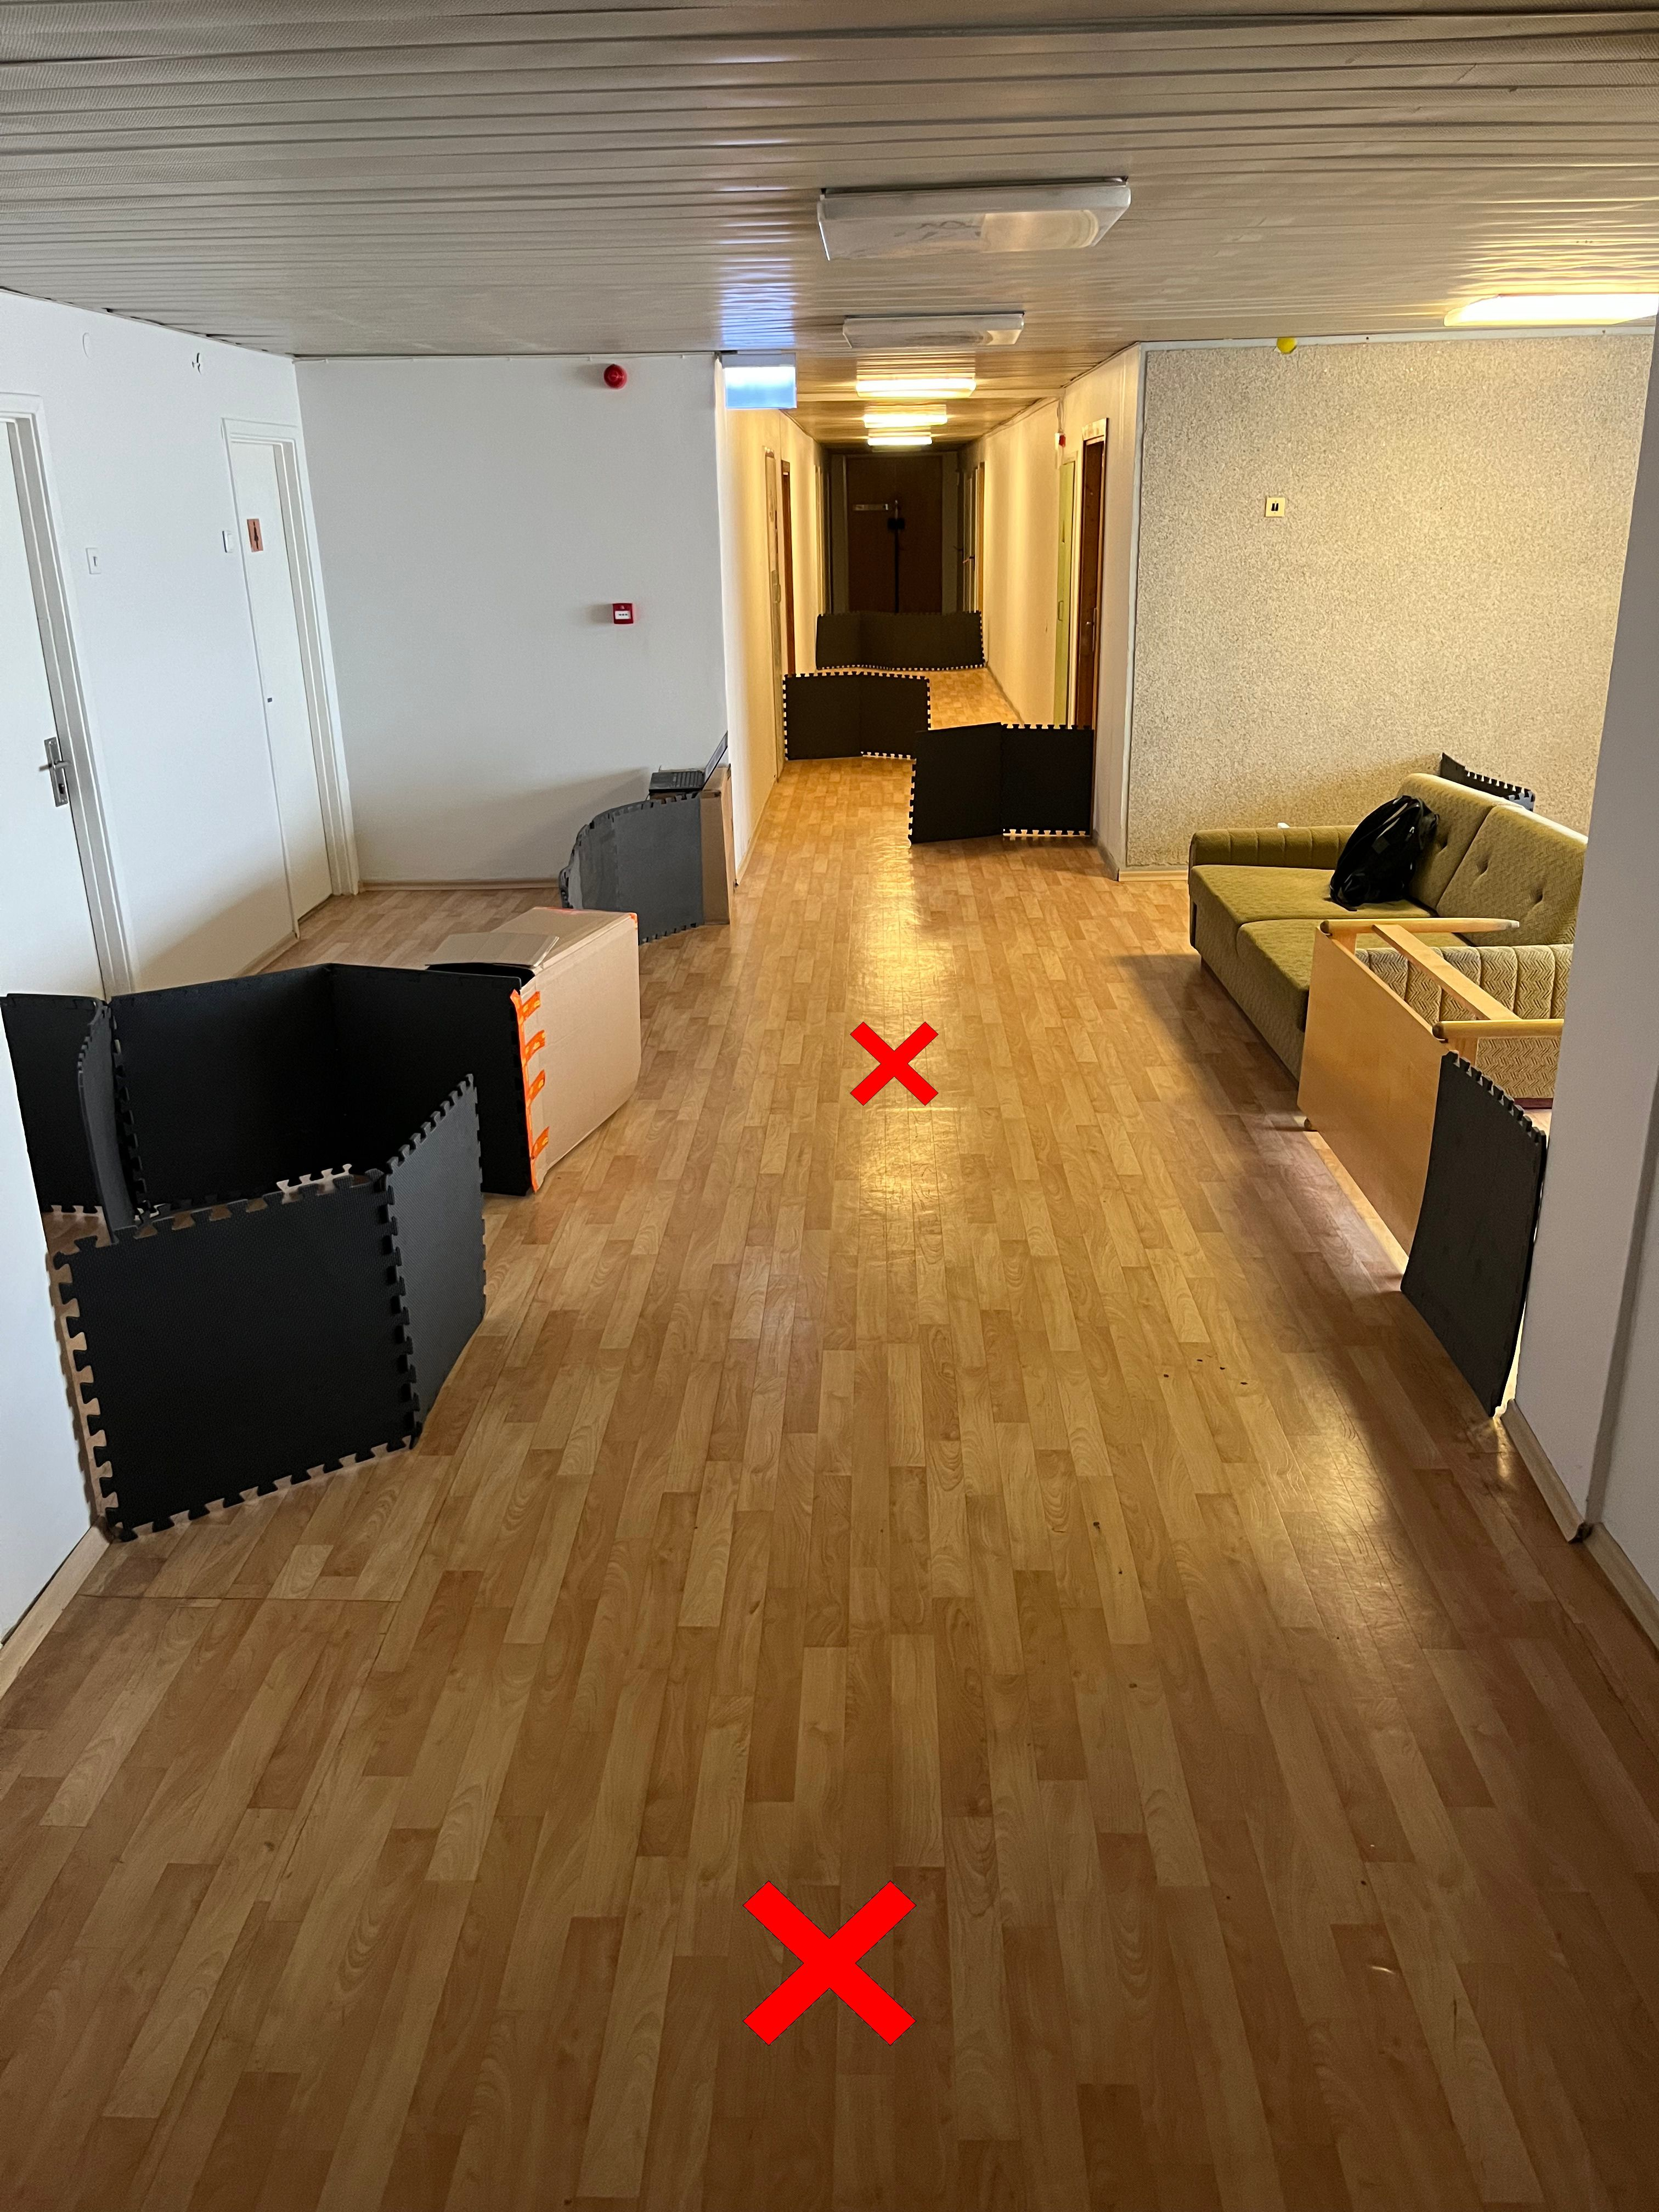
\includegraphics[height=0.37\textheight,width=\textwidth,keepaspectratio]{images/final/kamb3_marks.jpg}
            \caption{\scriptsize Ilgas koridorius}
        \end{figure}
    \end{columns}

    \vspace{0.15cm}
    \begin{itemize}
        \item 1 ir 2 aplinkose kiekvienas algoritmas vykdytas po 4 kartus.
        \item 3 aplinkoje kiekvienas algoritmas vykdytas po 3 kartus.
    \end{itemize}
\end{frame}

% 7. Metrikos
\begin{frame}{Vertinimo metrikos}
    \begin{columns}[onlytextwidth]
        \column{0.52\textwidth}
        \textbf{Pagrindinės metrikos:}
        \begin{itemize}
            \item išžvalgymo trukmė;
            \item žemėlapio padengimas;
            \item nuvažiuotas kelias;
            \item išsiųsti, pasiekti ir nepavykę navigacijos tikslai.
        \end{itemize}
        \column{0.45\textwidth}
        \textbf{Papildomos metrikos:}
        \begin{itemize}
            \item procesoriaus naudojimas;
            \item atminties naudojimas.
        \end{itemize}

        \smallgap
        \textbf{Pabaigos sąlyga:} 8 ciklai iš eilės be naujo tinkamo tikslo.
    \end{columns}
\end{frame}

% 8. Pirma aplinka
\begin{frame}{Rezultatai: pirma aplinka}
    \begin{columns}[onlytextwidth]
        \column{0.68\textwidth}
        \begin{table}
            \centering
            \tiny
            \begin{tabular}{lcccccc}
                \toprule
                \textbf{Algoritmas} & \textbf{n} & \textbf{Laik., s} & \textbf{Pad., \%} & \textbf{Kel., m} & \textbf{Tikslai} & \textbf{Nep.} \\
                \midrule
                BFS & 4 & 244,4 & \metricbest{96,6} & 17,26 & 11,5 & 1,0 \\
                Art. riba & 4 & 207,9 & 95,2 & \metricbest{14,77} & 9,0 & 1,0 \\
                Inf. pr. & 4 & 242,2 & 95,3 & 18,01 & 8,8 & 2,5 \\
                RRT & 4 & 202,2 & 95,0 & 16,43 & 7,5 & 0,8 \\
                Voronoi & 4 & \metricbest{200,9} & 95,2 & 17,40 & 6,8 & \metricbest{0,5} \\
                \bottomrule
            \end{tabular}
        \end{table}

        \begin{table}
            \centering
            \tiny
            \begin{tabular}{lcccc}
                \toprule
                \textbf{Alg.} & \textbf{Laikas, s} & \textbf{Pad., \%} & \textbf{Kelias, m} & \textbf{Nep.} \\
                \midrule
                BFS & 165,8--315,7 & 95,2--99,8 & 13,24--21,10 & 0--3 \\
                Art. riba & 137,2--263,2 & 95,0--95,5 & 11,10--17,45 & 0--3 \\
                Inf. pr. & 215,2--291,1 & 95,2--95,6 & 15,19--22,09 & 0--4 \\
                RRT & 134,4--245,4 & 94,5--95,6 & 11,72--25,15 & 0--2 \\
                Voronoi & 163,4--238,4 & 95,2--95,4 & 12,74--19,45 & 0--2 \\
                \bottomrule
            \end{tabular}
        \end{table}
        \column{0.3\textwidth}
        \begin{figure}
            \centering
            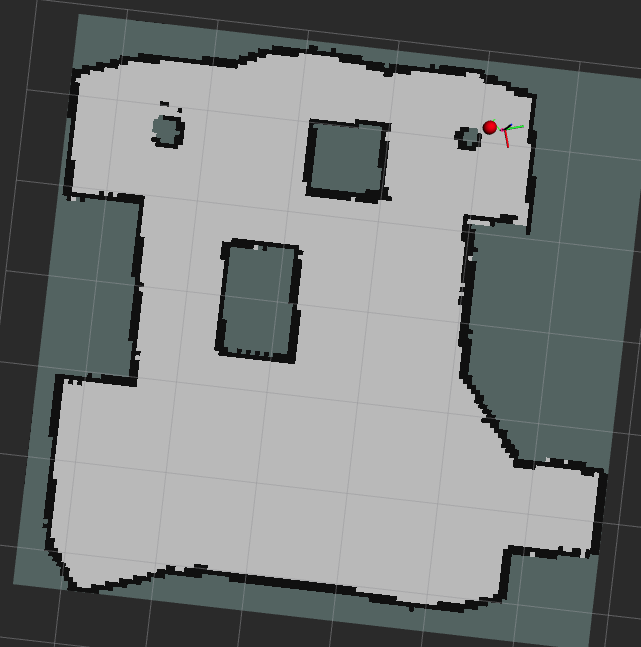
\includegraphics[width=\textwidth]{images/final/1_kamb_map.png}
            \caption{\scriptsize Žemėlapio pavyzdys}
        \end{figure}
    \end{columns}
\end{frame}

% 9. Antra aplinka
\begin{frame}{Rezultatai: antra aplinka}
    \begin{columns}[onlytextwidth]
        \column{0.68\textwidth}
        \begin{table}
            \centering
            \tiny
            \begin{tabular}{lcccccc}
                \toprule
                \textbf{Algoritmas} & \textbf{n} & \textbf{Laik., s} & \textbf{Pad., \%} & \textbf{Kel., m} & \textbf{Tikslai} & \textbf{Nep.} \\
                \midrule
                BFS & 4 & 358,7 & 98,4 & 20,02 & 19,3 & 3,0 \\
                Art. riba & 4 & \metricbest{162,1} & 98,4 & 13,79 & 11,0 & \metricbest{0,0} \\
                Inf. pr. & 4 & 172,8 & 98,4 & \metricbest{13,56} & 10,7 & \metricbest{0,0} \\
                RRT & 4 & 203,4 & 98,3 & 17,62 & 9,3 & 1,0 \\
                Voronoi & 4 & 224,7 & \metricbest{98,5} & 18,67 & 10,3 & 1,0 \\
                \bottomrule
            \end{tabular}
        \end{table}

        \begin{table}
            \centering
            \tiny
            \begin{tabular}{lcccc}
                \toprule
                \textbf{Alg.} & \textbf{Laikas, s} & \textbf{Pad., \%} & \textbf{Kelias, m} & \textbf{Nep.} \\
                \midrule
                BFS & 179,8--492,7 & 97,6--98,8 & 10,99--29,35 & 0--6 \\
                Art. riba & 146,1--181,1 & 98,4--98,4 & 11,35--17,15 & 0--0 \\
                Inf. pr. & 138,1--218,1 & 98,0--98,6 & 11,90--16,48 & 0--0 \\
                RRT & 140,4--245,3 & 97,8--98,6 & 11,34--25,00 & 0--2 \\
                Voronoi & 183,4--280,3 & 98,4--98,6 & 16,66--21,55 & 0--4 \\
                \bottomrule
            \end{tabular}
        \end{table}
        \column{0.3\textwidth}
        \begin{figure}
            \centering
            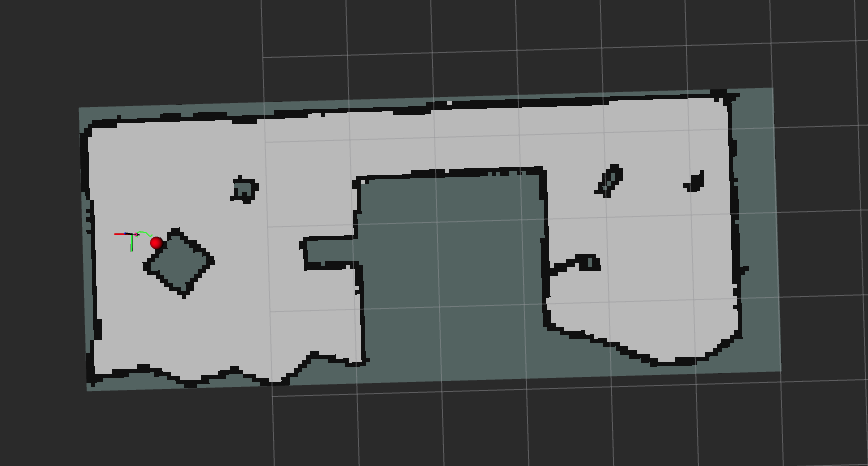
\includegraphics[width=\textwidth]{images/final/2_kamb_map.png}
            \caption{\scriptsize Žemėlapio pavyzdys}
        \end{figure}
    \end{columns}
\end{frame}

% 10. Trečia aplinka
\begin{frame}{Rezultatai: trečia aplinka}
    \begin{columns}[onlytextwidth]
        \column{0.68\textwidth}
        \begin{table}
            \centering
            \tiny
            \begin{tabular}{lcccccc}
                \toprule
                \textbf{Algoritmas} & \textbf{n} & \textbf{Laik., s} & \textbf{Pad., \%} & \textbf{Kel., m} & \textbf{Tikslai} & \textbf{Nep.} \\
                \midrule
                BFS & 3 & 533,6 & \metricbest{100,0} & 37,74 & 40,0 & 1,7 \\
                Art. riba & 3 & 342,9 & 99,9 & 31,69 & 19,7 & 3,0 \\
                Inf. pr. & 3 & \metricbest{259,1} & \metricbest{100,0} & \metricbest{27,28} & 12,0 & \metricbest{0,3} \\
                RRT & 3 & 418,7 & 99,7 & 38,42 & 21,3 & 4,0 \\
                Voronoi & 3 & 567,9 & \metricbest{100,0} & 54,50 & 23,0 & 5,7 \\
                \bottomrule
            \end{tabular}
        \end{table}

        \begin{table}
            \centering
            \tiny
            \begin{tabular}{lcccc}
                \toprule
                \textbf{Alg.} & \textbf{Laikas, s} & \textbf{Pad., \%} & \textbf{Kelias, m} & \textbf{Nep.} \\
                \midrule
                BFS & 367,6--683,5 & 100,0--100,0 & 32,58--41,29 & 0--5 \\
                Art. riba & 258,5--488,5 & 99,6--100,0 & 27,89--36,79 & 0--6 \\
                Inf. pr. & 226,4--282,4 & 99,9--100,0 & 22,88--32,83 & 0--1 \\
                RRT & 239,5--680,7 & 99,5--99,8 & 23,35--59,13 & 0--12 \\
                Voronoi & 387,5--697,2 & 99,9--100,0 & 37,81--65,06 & 4--7 \\
                \bottomrule
            \end{tabular}
        \end{table}
        \column{0.3\textwidth}
        \begin{figure}
            \centering
            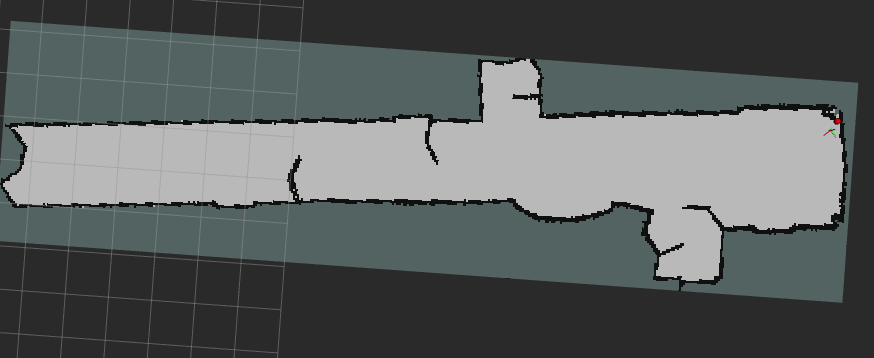
\includegraphics[width=\textwidth]{images/final/3_kamb_map.png}
            \caption{\scriptsize Žemėlapio pavyzdys}
        \end{figure}
    \end{columns}
\end{frame}

% 11. Rezultatų sklaida
\begin{frame}{Rezultatų sklaida}
    \begin{table}
        \centering
        \tiny
        \begin{tabular}{llcc}
            \toprule
            \textbf{Aplinka} & \textbf{Algoritmas} & \textbf{Laiko nuokrypis, s} & \textbf{Kelio nuokrypis, m} \\
            \midrule
            1 & BFS & 61,9 & 3,22 \\
            1 & Art. riba & 64,4 & 3,29 \\
            1 & Inf. pr. & 33,5 & \metricbest{3,17} \\
            1 & RRT & 50,7 & 5,96 \\
            1 & Voronoi & \metricbest{30,7} & 3,18 \\
            \midrule
            2 & BFS & 161,2 & 9,18 \\
            2 & Art. riba & \metricbest{17,7} & 3,01 \\
            2 & Inf. pr. & 41,1 & \metricbest{2,53} \\
            2 & RRT & 55,5 & 6,90 \\
            2 & Voronoi & 50,0 & 2,56 \\
            \midrule
            3 & BFS & 158,6 & \metricbest{4,57} \\
            3 & Art. riba & 126,6 & 4,59 \\
            3 & Inf. pr. & \metricbest{29,2} & 5,07 \\
            3 & RRT & 232,0 & 18,54 \\
            3 & Voronoi & 161,0 & 14,62 \\
            \bottomrule
        \end{tabular}
    \end{table}
\end{frame}

% 12. Nepavykę tikslai ir ištekliai
\begin{frame}{Nepavykę tikslai ir ištekliai}
    \begin{columns}[onlytextwidth]
        \column{0.52\textwidth}
        \begin{table}
            \centering
            \tiny
            \begin{tabular}{lccc}
                \toprule
                \textbf{Bandymas} & \textbf{Trukmė, s} & \textbf{Nep.} & \textbf{Dalis, \%} \\
                \midrule
                BFS, 1 apl., 1 band. & 315,7 & 3 & 60 \\
                BFS, 2 apl., 2 band. & 403,7 & 6 & 94 \\
                RRT, 3 apl., 1 band. & 680,7 & 12 & 111 \\
                Voronoi, 3 apl., 1 band. & 697,2 & 6 & 54 \\
                Voronoi, 3 apl., 3 band. & 619,0 & 7 & 71 \\
                \bottomrule
            \end{tabular}
        \end{table}
        \column{0.43\textwidth}
        \begin{table}
            \centering
            \scriptsize
            \begin{tabular}{lc}
                \toprule
                \textbf{Algoritmai} & \textbf{Vid. RAM} \\
                \midrule
                BFS, art. riba, inf. pr., RRT & 66--67 MB \\
                Voronoi & 96,2 MB \\
                \bottomrule
            \end{tabular}
        \end{table}
    \end{columns}
\end{frame}

% 13. Bendras palyginimas
\begin{frame}{Bendras palyginimas}
    \begin{columns}[onlytextwidth]
        \column{0.52\textwidth}
        \begin{center}
        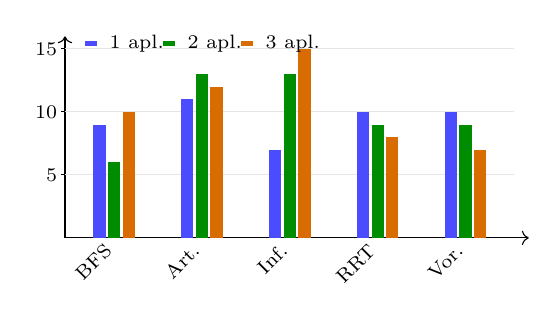
\begin{tikzpicture}[x=0.62cm,y=0.16cm]
            \scriptsize
            \draw[->] (0,0) -- (0,16);
            \draw[->] (0,0) -- (9.5,0);
            \foreach \y in {5,10,15} {
                \draw (-0.08,\y) -- (0,\y) node[left] {\y};
                \draw[gray!20] (0,\y) -- (9.2,\y);
            }
            \foreach \x/\name in {1/BFS,2.8/Art.,4.6/Inf.,6.4/RRT,8.2/Vor.} {
                \node[rotate=45,anchor=east] at (\x,-0.3) {\name};
            }
            \foreach \x/\a/\b/\c in {1/9/6/10,2.8/11/13/12,4.6/7/13/15,6.4/10/9/8,8.2/10/9/7} {
                \fill[blue!70] (\x-0.42,0) rectangle ++(0.25,\a);
                \fill[green!55!black] (\x-0.12,0) rectangle ++(0.25,\b);
                \fill[orange!85!black] (\x+0.18,0) rectangle ++(0.25,\c);
            }
            \fill[blue!70] (0.4,15.2) rectangle ++(0.25,0.45); \node[right] at (0.75,15.42) {1 apl.};
            \fill[green!55!black] (2.0,15.2) rectangle ++(0.25,0.45); \node[right] at (2.35,15.42) {2 apl.};
            \fill[orange!85!black] (3.6,15.2) rectangle ++(0.25,0.45); \node[right] at (3.95,15.42) {3 apl.};
        \end{tikzpicture}
        \end{center}
        \vspace{-0.15cm}
        \centering
        \scriptsize Rangavimo taškai pagal laiką, padengimą ir kelią
        \column{0.44\textwidth}
        \begin{table}
            \centering
            \scriptsize
            \begin{tabular}{lcc}
                \toprule
                \textbf{Algoritmas} & \textbf{Taškai} & \textbf{Vieta} \\
                \midrule
                Artimiausia riba & \metricbest{36} & \metricbest{1} \\
                Informacijos prieaugis & 35 & 2 \\
                RRT & 27 & 3 \\
                Voronoi & 26 & 4 \\
                BFS & 25 & 5 \\
                \bottomrule
            \end{tabular}
        \end{table}
    \end{columns}
\end{frame}

% 14. Išvados
\begin{frame}{Išvados (1)}
    \scriptsize
    \begin{enumerate}
        \item Penki skirtingų išžvalgymo strategijų grupių algoritmai palyginti vienoje realaus TurtleBot Burger roboto sistemoje, naudojant tas pačias programinės įrangos, navigacijos ir eksperimentinių aplinkų sąlygas.
        \item BFS daugeliu atvejų pasiekė aukštą padengimą, tačiau dažnai reikalavo daugiau navigacijos tikslų ir ilgesnio išžvalgymo laiko.
        \item Artimiausios ribos algoritmas pasižymėjo stabilumu visose aplinkose: antrojoje aplinkoje veikė greičiausiai ir neturėjo nepavykusių tikslų, pirmojoje pasiekė trumpiausią vidutinį kelią.
        \item Informacijos prieaugio algoritmas visose trijose aplinkose pasiekė gerus rezultatus, o ilgo koridoriaus aplinkoje buvo efektyviausias pagal laiką, kelią, padengimą ir nepavykusius tikslus.
        \item RRT algoritmas parodė didesnį rezultatų kintamumą: kai kuriais bandymais veikė greitai, tačiau sudėtingesnėse arba ištęstose aplinkose galėjo sugeneruoti ilgesnį kelią ir daugiau nepavykusių tikslų.
    \end{enumerate}
\end{frame}

% 15. Išvados
\begin{frame}{Išvados (2)}
    \scriptsize
    \begin{enumerate}
        \setcounter{enumi}{5}
        \item Voronoi algoritmas pirmoje aplinkoje veikė gerai, tačiau trečiojoje turėjo didžiausią vidutinį kelią ir daugiausia nepavykusių tikslų iš visų algoritmų.
        \item Galutinis žemėlapio padengimas nėra pakankama metrika: algoritmai dažnai pasiekė panašų padengimą, bet skyrėsi laiku, keliu ir nepavykusių tikslų skaičiumi.
        \item Standartinis nuokrypis parodė, kad geriausias vidutinis rezultatas ne visada reiškia vienodą stabilumą visose aplinkose; ilgame koridoriuje išryškėjo didesnė RRT ir Voronoi rezultatų sklaida.
        \item Paprastoms ir vidutinio sudėtingumo patalpoms galima rekomenduoti artimiausios ribos arba informacijos prieaugio metodus, o ilgesnėms koridoriaus tipo aplinkoms tinkamiausias buvo informacijos prieaugio algoritmas.
    \end{enumerate}
\end{frame}

% 16. Klausimai
\begin{frame}
    \begin{center}
        \Huge Ačiū už dėmesį
    \end{center}
\end{frame}

\end{document}
